\chapter{High Intensity Studies}
\label{sec:ch6}

\section{Global RDTs and Intensity-Dependent Effects}
\cite{mionrr}
\section{Space Charge Tune Shift}

\begin{equation}
    \Delta \nu_{sc}=\frac{-3 N r_0 R S}{4 \sigma_z M \beta \gamma ^2 \varepsilon_{N,95\%}}    
\end{equation}

\section{Measurement of Tune Spread}

% \newpage
% \begin{figure}[H]
%     \centering
%     \includegraphics[height=\textheight,keepaspectratio]{chapter6/scts_measure.png}
%     \caption{Tune spread.}
%     \label{fig:dynamictunespread}
% \end{figure}
% \newpage

\begin{figure}[H]
    \centering
    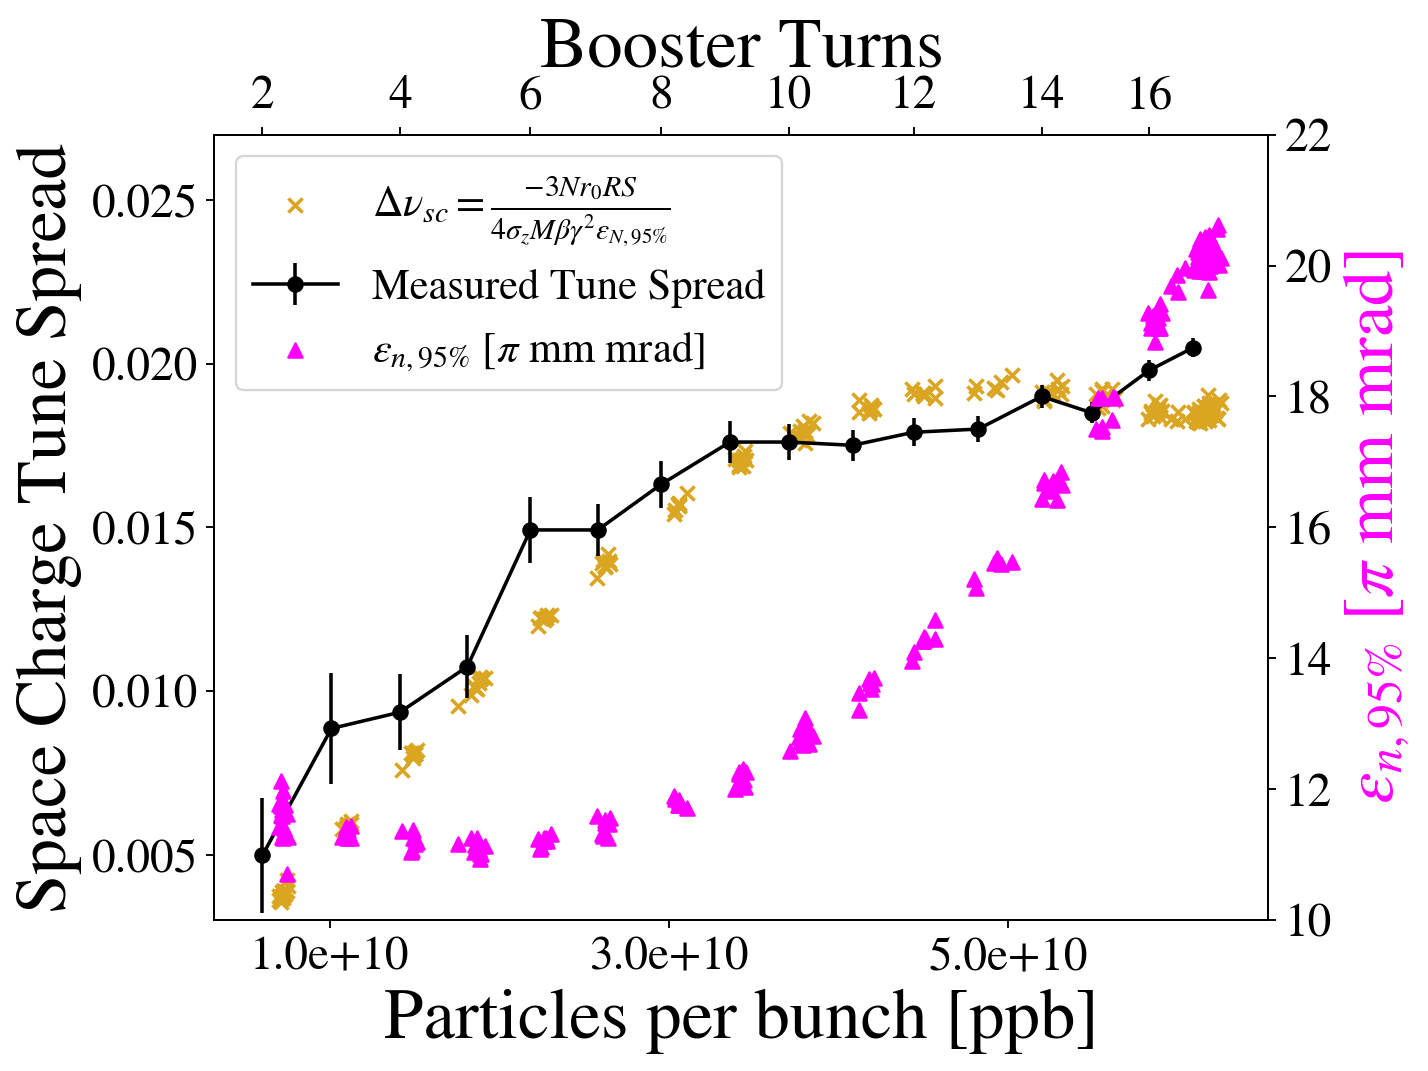
\includegraphics[width=\columnwidth]{chapter6/tune_spread.png}
    \caption{Measurement of tune spread.}
    \label{fig:tunespread}
\end{figure}

\section{Static Tune Scans at Different Intensities}

\begin{figure}[H]
    \centering
    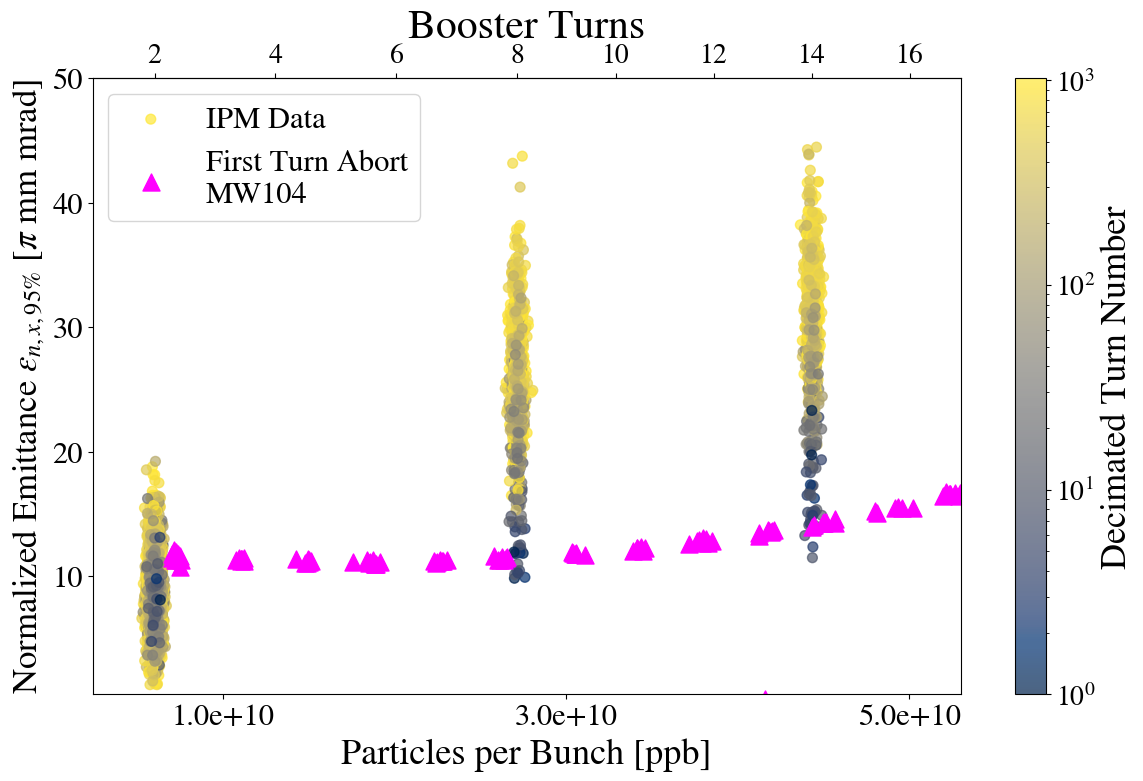
\includegraphics[width=\columnwidth]{chapter6/25370_scatter.png}
    \caption{IPM data and multi-wire first turn abort data for $Q_x=25.370$ at different intensities.}
    \label{fig:25370_scatter}
\end{figure}


\section{Effect of Transverse Dampers}

\begin{figure}[H]
    \centering
    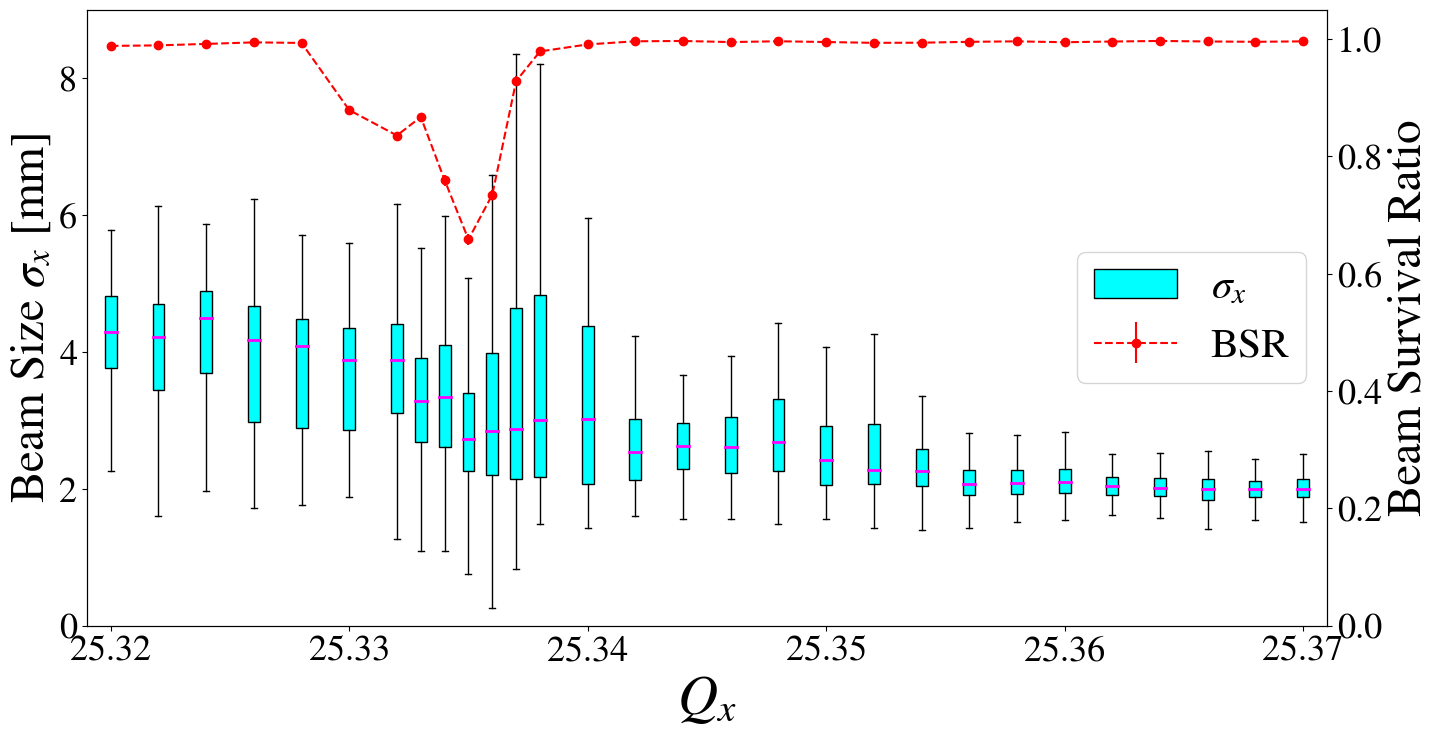
\includegraphics[width=\columnwidth]{chapter6/static2turns_ipm_dampersON.png}
    \caption{Static tune scan with beam survival ratio and IPM data box plots with $3Q_x$ compensation, transverse dampers ON and 2 Booster Turns of equivalent intensity.}
    \label{fig:static2_dampersON}
\end{figure}

\begin{figure}[H]
    \centering
    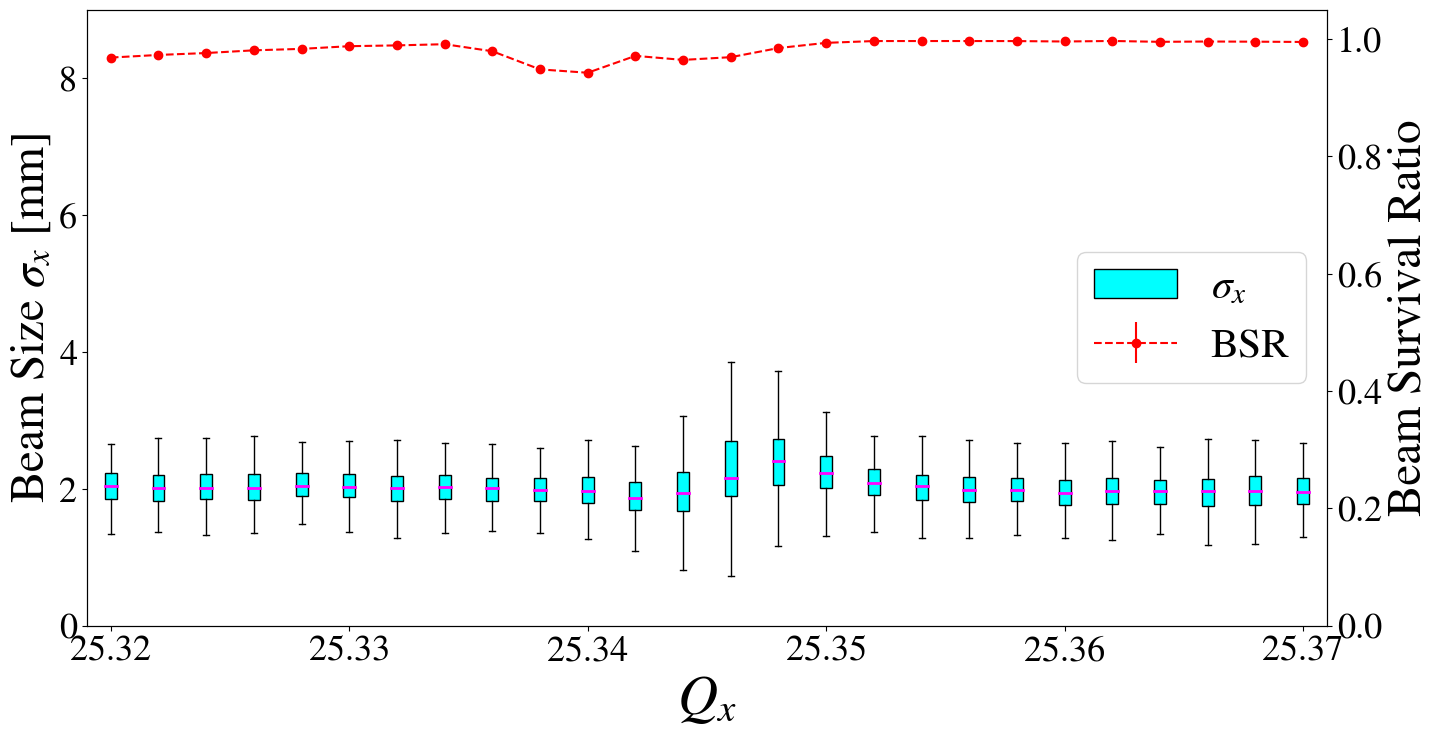
\includegraphics[width=\columnwidth]{chapter6/static2turns_ipm_dampersOFF.png}
    \caption{Static tune scan with beam survival ratio and IPM data box plots with $3Q_x$ compensation, transverse dampers OFF and 2 Booster Turns of equivalent intensity.}
    \label{fig:static2_dampersOFF}
\end{figure}

